\chapter{Analysis}
\label{chap:analysis}
\epigraph{``The trouble with writing fiction is that it has to make sense, whereas real life doesn't"}{--- \textup{Iain M. Banks}}

The purpose of this chapter is to compare the BIS data structure to the kd-tree. We are going to perform a variety of tests on the BIS data structure and the kd-tree in order to determine the run-time properties of both, mainly looking at when the BIS data structure performs better than the kd-tree.\\


Random data will be generated and given as input to the data structures. Both data structures will be given the same random data. This way they operate on the some data and the comparison will be fair. The random data is generated by making two lists, $X$ and $Y$ with the integers $[0,n-1]$ and shuffling them both randomly. The $n$ points given to the data structures as input are found by taking the $i$th entry of both $X$ and $Y$ and generating a point with those coordinates. This ensures that all x-coordinates are unique and all y-coordinates are unique. When running a specific test, different data sets will be generated and given as new input to the data structures such that a test is not only performed on a single data set. The different tests will check how a given shape impacts the running time of a query to the data structures. When the shape and size of the search query has been determined, the search will performed with a different displacement on the x-axis and y-axis such that the queries are performed all over the data structure and not only in a best-case or worst-case position. The search query is performed a lot of times and then the average time per query is returned.

We are mainly going to focus on two different kinds of tests. First we are going to test how a search query shaped like a square performs in both the BIS data structure and the kd-tree. This type of query will be good for the kd-tree since it will get to fully include many regions. In the second test the configuration of the search query is going to one where the worst-case scenario for the kd-tree happens. It will cover the entirety of the search area in a thin slice either in a vertical or horizontal direction. In the third section we are going to look closer at how much better the search query to the SRS data structure compares to the search query to the kd-tree when the search query is a vertical or horizontal slice and $k \leq 200$. The limit of $200$ is chosen based because it is small and a reasonable amount of results for human interaction.

The tests have been performed on data structures with data sets of size $2^{\lg n}$ where $\lg n = [17,25]$. $17$ was chosen as the smallest because it would still be big enough to show something interesting on the graphs. $25$ was chosen because the current initialization of the SRS data structure requires a bit of work and thus takes up nearly all of the main memory. Future work includes an idea for a faster and less memory requiring setup phase.

In all the test we have chosen $B = \lceil \frac{1}{2}\lg^{\frac{1}{3}} n \rceil$. Recall from section~\ref{ssection:fasterqueries} that $B = \Omega(\lg^\epsilon n)$. Thus, we have chosen $\epsilon = \frac{1}{3}$. Section~\ref{ssection:fasterqueries} also states that $B$ is responsible for the big jumps in the ball inheritance structure: where the jumps should be placed and how big they should be. Unless otherwise stated the graphs in this chapter show results from a BIS data structure configured with $B = \lceil \frac{1}{2}\lg^{\frac{1}{3}} n \rceil$.



\section{Square search queries}
\label{sect:squares}

This section will show the running time of square search queries to both data structure. With this configuration we expect to see that kd-tree performs better than the BIS data structure. We are interested in seeing just how much worse the BIS data structure performs. 

\subsection{Setup}
The kd-tree has a query time of $\mathcal{O}(\sqrt{n}+k)$. The $\sqrt{n}$ part is based on a pessimistic notion that an edge of a query will pass through the entire search area of the kd-tree. This is not always the case. We also note that when $k > \sqrt{n}$, $k$ will dominate the expression and thus the query time will be linear. In order to fairly compare the running time of a search query to both data structure, we are going to generate queries finding the points within an area of $\sqrt{size}\cdot\sqrt{n} \times \sqrt{size}\cdot\sqrt{n}$ where size will increase. As previously described, this search query will be made with random displacements in order to query arbitrary places in the structures. So given two random numbers $x$ and $y$ a query will be $q = [x, x+\sqrt{size}\cdot\sqrt{n}] \times [y, y+\sqrt{size}\cdot\sqrt{n}]$. A query of this shape will not invoke the worst-case scenario for the kd-tree and will thus give an idea of how the BIS data structure performs in contrast to the kd-tree under circumstances where the kd-tree performs well. 

The points generated for the data structures lie in the range of $[0,n-1] \times [0,n-1]$, which gives an area of $n^2$. If the search query has an area of $A$, each point has a $\frac{A}{n^2}$ chance of being in that search query. With $n$ points we thus expect to find $n\cdot \frac{A}{n^2}$ points in a search query with the area of $A$. In this test we set $A = \sqrt{n}\cdot\sqrt{size}\times\sqrt{n}\cdot\sqrt{size}$, where $n$ is constant to the data structure and $size$ will increase during the test. We then expect to find $n\cdot\frac{A}{n^2} = \frac{n\cdot n \cdot size}{n^2} = size$ points. This obviously depends a lot on how the points are distributed in that specific case. When generating $10$ different data sets for the data structures in the tests and picking the displacements for the search query at random each search, we will expect the average amount of points returned by the search query $q = [x, x+\sqrt{size}\cdot\sqrt{n}] \times [y, y+\sqrt{size}\cdot\sqrt{n}]$ to be $size$.

\subsection{Data}

One thing to notice is that the running time of a query increases linear to the amount of points returned. This agrees with the theoretical running time of $\mathcal{O}(\lg n + k\cdot \lg^\epsilon n)$. The theoretical $\mathcal{O}(\lg^\epsilon n)$ is the worst-case amount of jumps from a any given node to a leaf. Looking at figure~\ref{fig:sqrt_25} we notice that around $size\approx 150$ the graph changes its slope. This means that the average amount of jumps per point reported back can change, but will naturally always be bounded by the worst-case of $\lg^\epsilon n$. Other factors may have a say in the change of slope as well. Some of these factors will be mentioned in section~\ref{sect:verthoriexp}.

As expected, the average amount of points reported from a lot of search queries with $q = [x, x + \sqrt{size}\cdot\sqrt{n}] \times [y, y + \sqrt{size}\cdot\sqrt{n}]$ were $size$.\todo{Kan jeg bare skrive det eller skal jeg vise en graf? Skal jeg skrive mere om det?}

The graphs below show the time of a search query to the SRS data structure compared to the time of a search query to the kd-tree. As described, the shape of the search query is a square. The variable $size$ increments in levels of $5$ per iteration of the test and will have a maximum of $\frac{\sqrt{n}}{2}$. The x-axis of the graphs describes the $size$ variable in the expression $A = \sqrt{n}\cdot\sqrt{size} \times \sqrt{n}\cdot\sqrt{size}$. Examining figure~\ref{fig:sqrt_17} we see that when the shape of the search query is a square, the search query to the kd-tree is always performing better than the search query to the SRS data structure. Looking closer at the figure we notice that while the search query to the SRS data structure performs worse, it is not that bad. At $size = 180$ we have window of size $\sqrt{2^{17}}\cdot\sqrt{180} \times \sqrt{2^{17}}\cdot\sqrt{180} = 4857.26 \times 4857.26$. The time to perform the search query on the SRS data structure at $size = 180$ is $15.9$ microseconds, while the search to the kd-tree takes $5.2$. This search query includes $180$ points. This is a relatively big query and the time to perform the search query on the SRS data structure is only a factor $3$ worse than the time of the search query on kd-tree.


This can have something to do with the different ways the SRS data structure and the kd-tree behaves given a search query. The kd-tree uses the actual search query in its normal form, $[x_1, x_2] \times [y_1, y_2]$ and compares that with the region of each node the search encounters. The first things the SRS data structure does given a search is to translate it into rank space. In rank space we know precisely how many points are in $[\hat{x_1}, \hat{x_2}]$ and $[\hat{y_1}, \hat{y_2}]$ and thus the search query is dependent on how many points are in $[\hat{x_1}, \hat{x_2}]$ and $[\hat{y_1}, \hat{y_2}]$ rather than how big the search query is. \todo{Det er måske også en trend vi kan kigge på med slices}

Examining figure~\ref{fig:sqrt_25} with $n = 2^{25}$ the largest search window has become quite large with a size of $\sqrt{2^{25}}\cdot\sqrt{2895} \times sqrt{2^{25}}\cdot\sqrt{2895} = 311673 \times 311673$. The biggest window now returns $2895$ points. A search query with this size to the SRS data structure and the search query to the kd-tree has a factor $\frac{386}{24} = 16.1$ difference. This a quite big difference in the search time, but it is also a big search query.

It is obvious from the graphs that the kd-tree performs better when the search queries are square windows. The time of a search query to the BIS data structure grows linearly to the size of the window, just like a query to the kd-tree, but with a bigger slope. This means you will not run into an unexpected growth when asking for more points from the BIS data structure.

The biggest search query at $n = 2^{17}$ is $\sqrt{180}\cdot{n} \times \sqrt{180}\cdot\sqrt{n}$. We now fix $size = 100 \leq 180$ and see how the ratio between the search query to the BIS data structure and kd-tree will evolve when $n$ grows. We see this on figure~\ref{fig:factdiffsqrt100}. The graph is growing and thus the running time of a search query to the BIS data structure returning the same amount of points when $n$ is growing increases faster than the same search query to the kd-tree.\todo{Skriv noget om hvordan det vokser for hvert $\lg n$. $n$ stiger med $2$, men grafen stiger lineært}

\begin{figure}[h]
  \makebox[\linewidth][c]{
    \centering
    \begin{subfigure}[b]{0.68\textwidth}
        \centering
        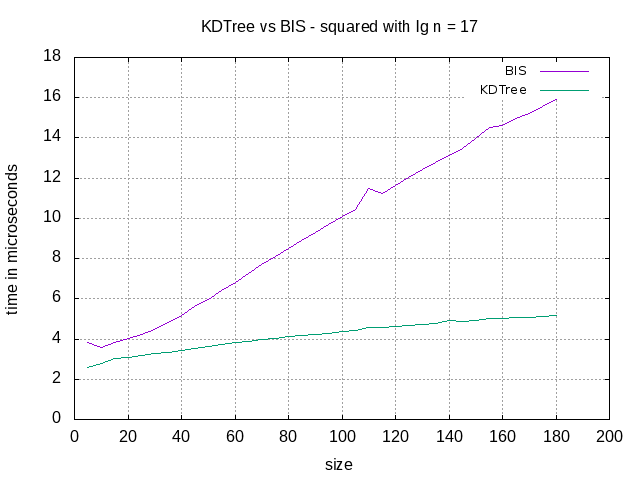
\includegraphics[width=0.99\textwidth]{pictures/analysis/sqrt_17.png}
        \caption{$n = 2^{17}$ with $\sqrt{n} = 362$.}
        \label{fig:sqrt_17}
    \end{subfigure}
    %\hfill
    \begin{subfigure}[b]{0.68\textwidth}
        \centering
        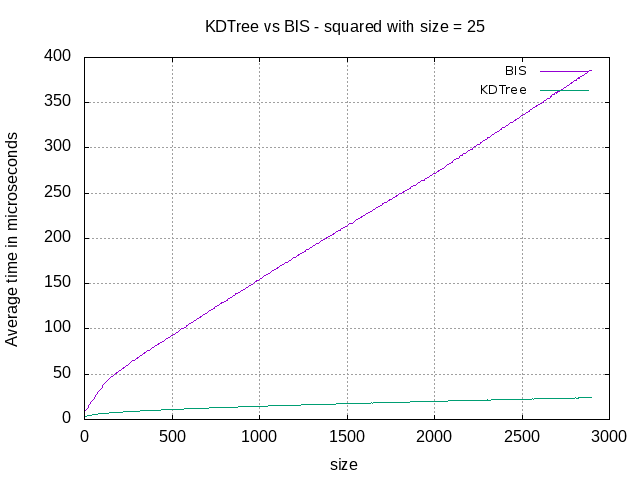
\includegraphics[width=0.99\textwidth]{pictures/analysis/sqrt_25.png}
        \caption{$n = 2^{25}$ with $\sqrt{n} = 5792$.}
        \label{fig:sqrt_25}
    \end{subfigure}
  }
    \caption{Square search on BIS and kd-tree.}
    \label{fig:sqrt_17_25}
  
\end{figure}

\begin{figure}[h]
    \centering
    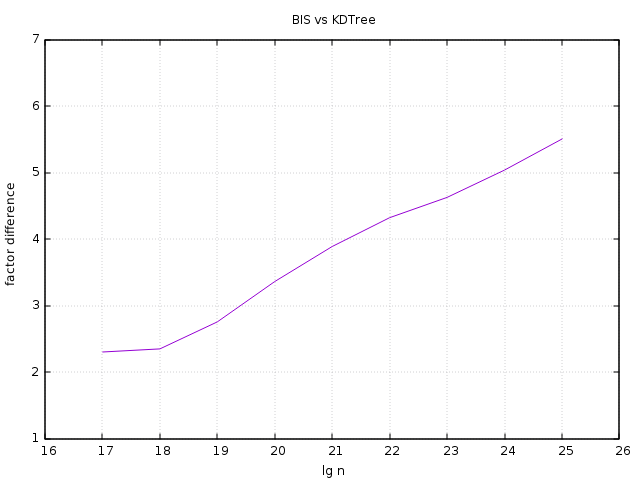
\includegraphics[width = 0.85\textwidth]{pictures/analysis/factor_difference_sqrtn_100.png}
    \caption{Ratio between a square query to the kd-tree and BIS data structure with constant $size = 100$. Ratio describes how much better the kd-tree performs.}\label{fig:factdiffsqrt100}
\end{figure}

\clearpage


\section{Vertical and horizontal slices}

In this section we are going to compare the performance of the BIS data structure and the performance of the kd-tree when the search query is in the shape of a \emph{slice}. We define a \emph{slice} to be a search query which covers the entirety of the search space in one dimension while only covering a small part of the search space in the other dimension. Since a slice is a search query with the form of either $q_h = [0, n-1] \times [y_1, y_2]$ or $q_v = [x_1, x_2] \times [0, n-1]$ we omit $[0, n-1]$ and define the \emph{size of the slice} to be $\left| y_2-y_1\right|$ or $\left|x_2-x_1\right|$. The way that the points for the data structures have been generated means that a slice of size $k$ will always return $k$ results.

\subsection{Setup}

A search query to the kd-tree has a run-time of $\mathcal{O}(\sqrt{n}+k)$ and a search query to the SRS data structure has a run-time of $\mathcal{O}(\lg n + k \cdot \lg^\epsilon n)$. We expect the run-time of a slice to the BIS to be faster when $k$ is small, but when $k$ gets bigger the kd-tree will be best. When increasing the size of a slice, we expect the run-time of the two search queries to be roughly equal at $k \approx \frac{\sqrt{n} - \lg n}{\lg^\epsilon n - 1}$ originating from $\sqrt{n} + k = \lg n + k \cdot \lg^\epsilon n \Leftrightarrow k = \frac{\sqrt{n} - \lg n}{\lg^\epsilon n - 1}$. We call this theoretical intersection point between the running times for $k_t$. The $\mathcal{O}(\lg^\epsilon n)$ bounds the amount of jumps needed to perform in order to find the identity of a leaf given the identity of a ball in the ball inheritance structure. In $k_t$ we will let $\lg^\epsilon n$ describe average amount of jumps taken by each point reported back as a result of the query, meassured by the experiments.

Recall that the SRS data structure treats the two dimensions very differently. Given a rank space search query $\hat{q} = [\hat{x_1}, \hat{x_2}] \times [\hat{y_1}, \hat{y_2}]$, the search algorithm will find the least common ancestor of $\hat{x_1}$ and $\hat{x_2}$. From there, it will find the path to both $\hat{x_1}$ and $\hat{x_2}$ and all leaves between them will be in the range $[x_1, x_2]$. The search algorithm now has to determine which of these leaves contain a point with y-coordinate in $[y_1, y_2]$. This is done by using the ball inheritance structure from each of the fully contained nodes which were found on the path from the least common ancestor to $\hat{x_1}$ and $\hat{x_2}$.

This means that a horizontal slice and a vertical slice will be treated differently by the SRS data structure. The search query of a horizontal slice includes all x-coordinates of the search space, and thus the least common ancestor of $[\hat{x_1}, \hat{x_2}]$ will be the root of the tree. The path from the least common ancestor to $\hat{x_1}$ will only go left which means each level will have one fully contained node. The path from the least common ancestor to $\hat{x_2}$ will only go right, also yielding one fully contained node per level. The tests measure the difference in performance between the BIS data structure and the kd-tree when the search query is a slice. A slice will start out being very small, $k=5$. Thus, many of the fully contained nodes will have no ball inheritance work when the slice is a horizontal slice. As the slice grows, eventually more and more node will have one or more balls to follow. The amount of ball inheritance each node is responsible for varies a lot, and therefore the ball inheritance will become somewhat sporadic. But the nature of the ball distribution asserts that if node has two balls or more balls for ball inheritance, these balls will be right next to each.

On the other hand we have the vertical slices. The vertical slice includes all y-coordinates of the search space, and thus the location of the least common ancestor of $[\hat{x_1}, \hat{x_2}]$ varies a lot dependent on the search query. But the nodes which are marked as fully contained on the path from the least common ancestor to $\hat{x_1}$ and $\hat{x_2}$ will all only contain leaves with points with y-coordinates in $[y_1, y_2]$ which means we have to do ball inheritance on all the balls belonging to fully contained nodes. Thus, the ball inheritance in vertical slices are much more batched together. Comparing a vertical and horizontal slice of the same size, the vertical slice will have good chances of being faster than the horizontal slice. With a lower LCA, the ball inheritance in the vertical slice will have to jump from a lower level than the ball inheritance in the horizontal and the balls are more batched together in the vertical. 

We are going to look at how well the vertical and horizontal slices perform on both the SRS data structure and the kd-tree. We are interested in seeing how big the slices can become before the search query to the BIS data structure performs worse than the serach query to the kd-tree. We are going to look at the vertical slices first. Below are some graphs showing the running time of a search query to both the SRS and the kd-tree dependent on the size of the slice. 

\subsection{Vertical slices}

Figures~\ref{fig:vert_17} and figure~\ref{fig:vert_25} show the performance of a search query to the BIS data structure compared to a search query to the kd-tree, where the search query is a vertical slice.


\begin{figure}[h]
  \makebox[\linewidth][c]{
    \centering
    \begin{subfigure}[b]{0.68\textwidth}
        \centering
        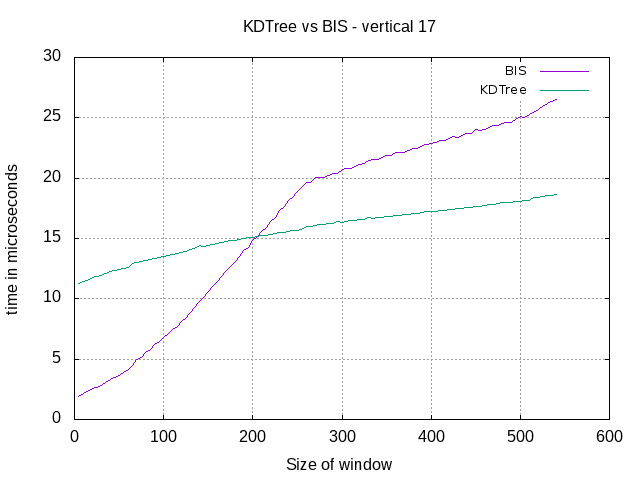
\includegraphics[width=0.99\textwidth]{pictures/analysis/vert_17.png}
        \caption{$n = 2^{17}$}
        \label{fig:vert_17}
    \end{subfigure}
    %\hfill
    \begin{subfigure}[b]{0.68\textwidth}
        \centering
        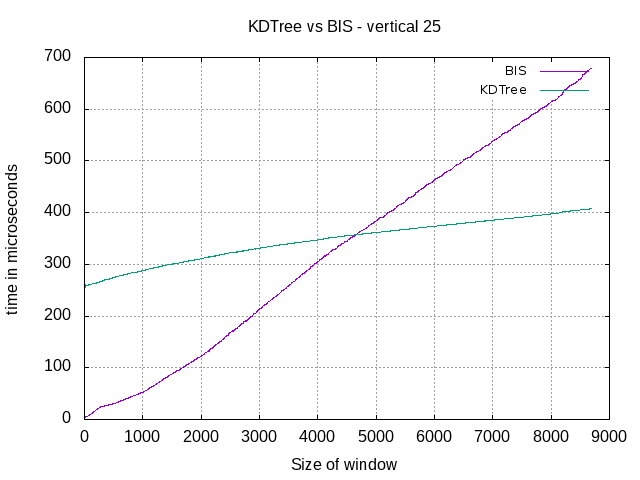
\includegraphics[width=0.99\textwidth]{pictures/analysis/vert_25.png}
        \caption{$n = 2^{25}$}
        \label{fig:vert_25}
    \end{subfigure}
  }
    \caption{Vertical slice on BIS and kd-tree.}
    \label{fig:vert_17_25}
  
\end{figure}

\clearpage


Figure~\ref{fig:vert_intersection} shows the size of the slice at the point of intersection between the running-time of a search to the BIS and the kd-tree for each $n$ tested. We can also see the intersection point for $\lg n = 17$ at figure~\ref{fig:vert_17} and for $\lg n = 25$ on figure~\ref{fig:vert_25}. Recall the theory described above where it was described how the intersection point should theoretically be $k_t = \frac{\sqrt{n} - \lg n}{\lg^\epsilon n - 1}$. Figure~\ref{fig:vert_theory} shows $\frac{k_m}{k_t}$, where $k_m$ is the amount of results meassured by the experiments. The graph is plotted using $\lg^\epsilon n$ as the average jumps per result. If the graph is below $1$ it means that the BIS data structure performed worse than theoretically expected and if it above $1$ it means that the BIS data structure performed better than theoretically expected. Except for $\lg n = 17$ at figure~\ref{fig:vert_theory} the figure shows that the BIS structures performs better, if only slightly, than we had theoretically expected. We also notice that the graph lies steadily around $1$ meaning that is a stable relationship. Figure~\ref{fig:vert_intersection} has a exponential tendency. That is to expected since the x-axis is $\lg n$ which means that $n$ grows by a factor of $2$ each step on the x-axis and then the point of intersection between the two running times increases by approximately $\sqrt{2}$. This is because of the $\mathcal{O}(\sqrt{n})$ part from the running time of a search query to the kd-tree. A slice is the worst-case scenario for the kd-tree. \todo{Måske lidt mere omkring det}

\begin{figure}[h]
  \makebox[\linewidth][c]{
    \centering
    \begin{subfigure}[b]{0.68\textwidth}
        \centering
        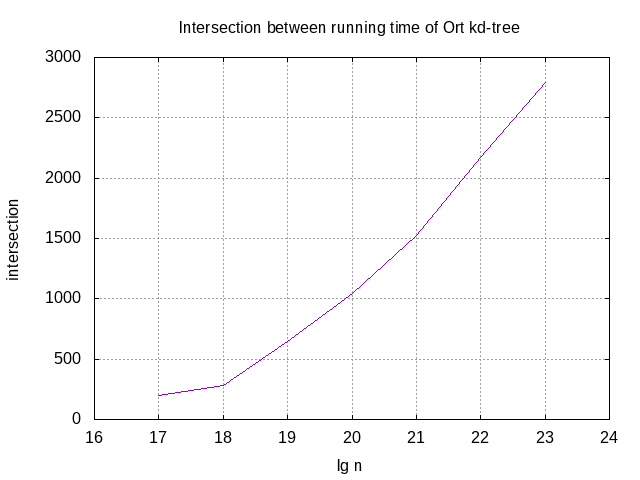
\includegraphics[width=0.99\textwidth]{pictures/analysis/vert.png}
        \caption{Point of intersection between BIS and kd-tree.}
        \label{fig:vert_intersection}
    \end{subfigure}
    %\hfill
    \begin{subfigure}[b]{0.68\textwidth}
        \centering
        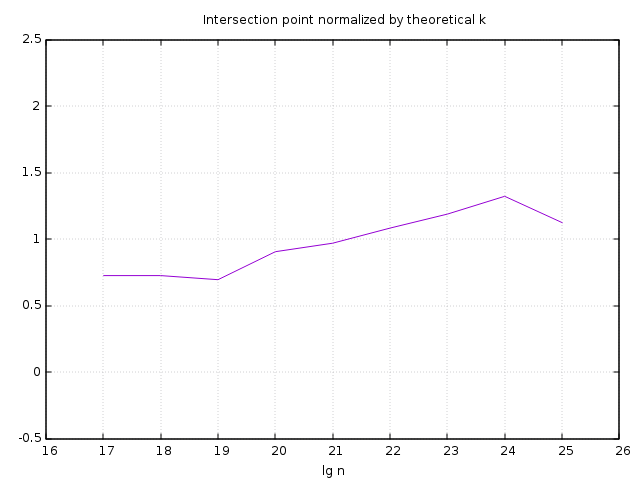
\includegraphics[width=0.99\textwidth]{pictures/analysis/vert_theory.png}
        \caption{Point of intersection normalized by theoretical $k$}
        \label{fig:vert_theory}
    \end{subfigure}
  }
    \caption{Vertical slice on BIS and kd-tree.}
    \label{fig:vert_intersection_and_theory}
  
\end{figure}
\clearpage


\subsection{Horizontal slices}

We are now going to look at the graphs for the horizontal slices. Recall that when a search query is a horizontal slice, the least common ancestor will be the root of the tree. In $[\hat{x_1}, \hat{x_2}]$, $\hat{x_1}$ will be the leftmost leaf and $\hat{x_2}$ will be the rightmost leaf. From the root to $\hat{x_1}$ and $\hat{x_2}$ there will many fully included nodes, $2$ per level to be exact, which means there will be many different nodes performing small amount of balls inheritance look-ups. Since the points are ordered by their y-coordinate in the root before distribution, and the fact that they keep this order while being distributed means that when increasing the range from $[y_1, y_2]$ to $[y_1, y_2 + 5]$ it is more likely that these $5$ new points will be found from a higher level where the range $[y_1, y_2]$ already had jumps from. It is much more likely that a point is stored in a leaf which belongs to a fully included node from level $8$ with $256$ leaves than it belongs to a node from level $2$ with $4$ leaves. Since the points are distributed to leaves according to their x-coordinates, it is hard to argue about the distribution of y-coordinates. The way the data has been generated, each x-coordinate has essentially been assigned a random y-coordinate and together they produce a point. When a search query is a horizontal slice, the position of $\hat{y_1}$ and $\hat{y_2}$ will be found on the bit vector of the root node. These positions will be updated using the succint rank query while traveling from the root node to the leftmost leaf and the rightmost leaf in the tree. \todo{Skriv om - distribution passer bedre end ordered}

Figures~\ref{fig:hori_17} and figure~\ref{fig:hori_25} show the performance of a search query to the BIS data structure compared to a search query to the kd-tree, where the search query is a horizontal slice.


\begin{figure}[h]
  \makebox[\linewidth][c]{
    \centering
    \begin{subfigure}[b]{0.68\textwidth}
        \centering
        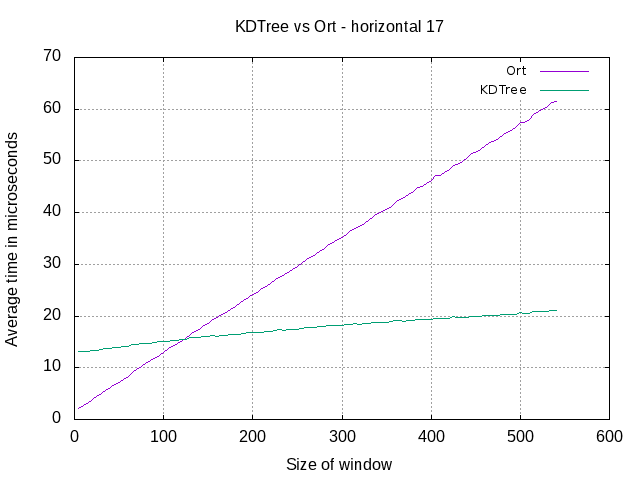
\includegraphics[width=0.99\textwidth]{pictures/analysis/hori_17.png}
        \caption{$n = 2^{17}$}
        \label{fig:hori_17}
    \end{subfigure}
    %\hfill
    \begin{subfigure}[b]{0.68\textwidth}
        \centering
        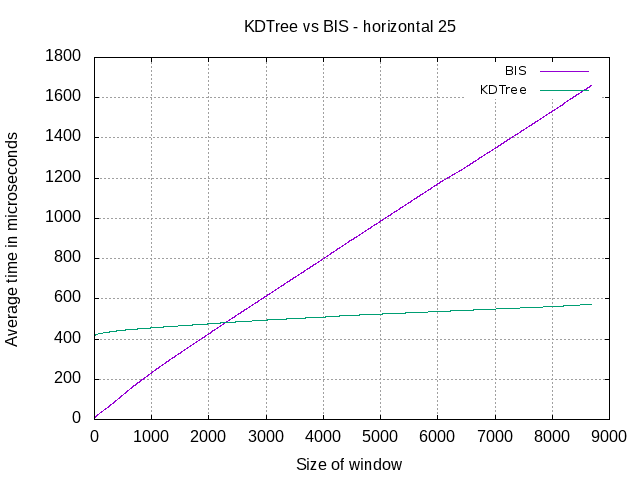
\includegraphics[width=0.99\textwidth]{pictures/analysis/hori_25.png}
        \caption{$n = 2^{25}$}
        \label{fig:hori_25}
    \end{subfigure}
  }
    \caption{Horizontal slice on BIS and kd-tree.}
    \label{fig:hori_17_25}
  
\end{figure}


Figure~\ref{fig:hori_intersection} shows the size of the slice at the point of intersection between the running-time of a search to the BIS and kd-tree for each $n$ tested. Figure~\ref{fig:hori_intersection} is a little more messy than figure~\ref{fig:vert_intersection} which is a point we will address in section~\ref{sect:verthoriexp}. At figure~\ref{fig:hori_theory} the graph crosses above and below $1$, but keeps rather close to $1$ which is the point where the performance is as we would theoretically expect. Again, we are looking for a graph that is as close to $1$ in order to show that is a stable relationship. 

\begin{figure}[h]
  \makebox[\linewidth][c]{
    \centering
    \begin{subfigure}[b]{0.68\textwidth}
        \centering
        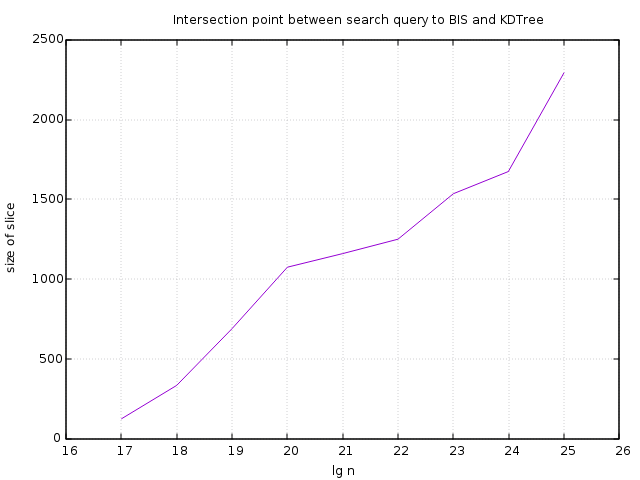
\includegraphics[width=0.99\textwidth]{pictures/analysis/hori.png}
        \caption{Point of intersection between BIS and kd-tree.}
        \label{fig:hori_intersection}
    \end{subfigure}
    %\hfill
    \begin{subfigure}[b]{0.68\textwidth}
        \centering
        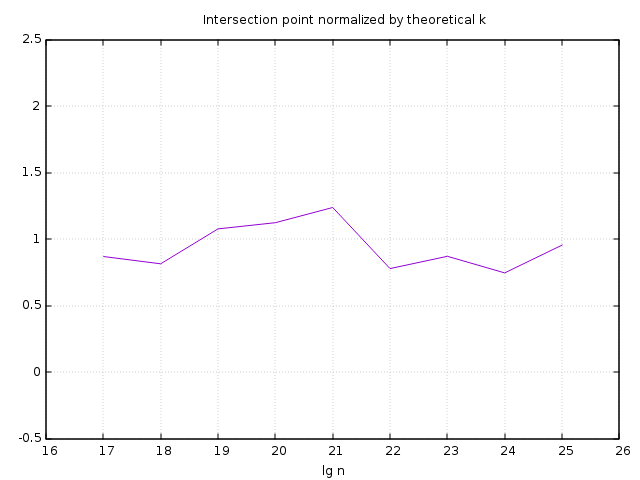
\includegraphics[width=0.99\textwidth]{pictures/analysis/hori_theory.png}
        \caption{Point of intersection normalized by theoretical $k$}
        \label{fig:hori_theory}
    \end{subfigure}
  }
    \caption{Horizontal slice on BIS and kd-tree.}
    \label{fig:hori_intersection_and_theory}
  
\end{figure}
\clearpage

\section{Comparision of SRS and kd-tree with a small $k$}
\label{sect:smallk}


In this section we are going to look at slices with $k\leq 200$. We will only focus on vertical slices. We are interested in seeing how much faster the SRS data structure is than the kd-tree when looking at amounts of results which seems reasonable to user interaction. Figure~\ref{fig:small_vert_17} figure~\ref{fig:small_vert_25} show the performance a search query to the BIS data structure compared to a search query to the kd-tree, where $k \leq 200$ for vertical slices.

\begin{figure}[h]
  \makebox[\linewidth][c]{
    \centering
    \begin{subfigure}[b]{0.68\textwidth}
        \centering
        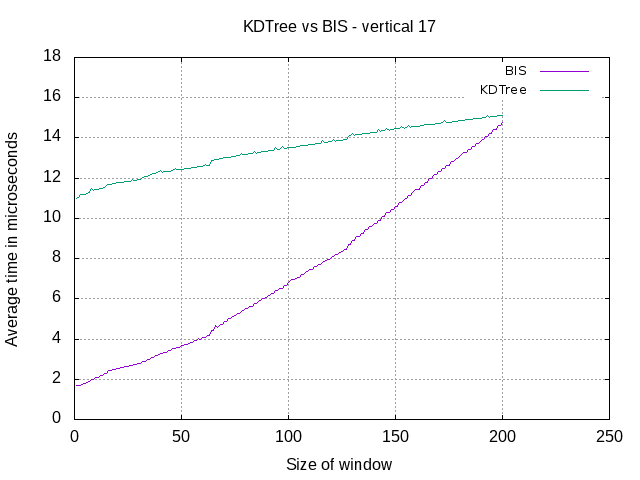
\includegraphics[width=0.99\textwidth]{pictures/analysis/smalls/vert_17.png}
        \caption{Data set of size $n=2^{17}$.}
        \label{fig:small_vert_17}
    \end{subfigure}
    %\hfill
    \begin{subfigure}[b]{0.68\textwidth}
        \centering
        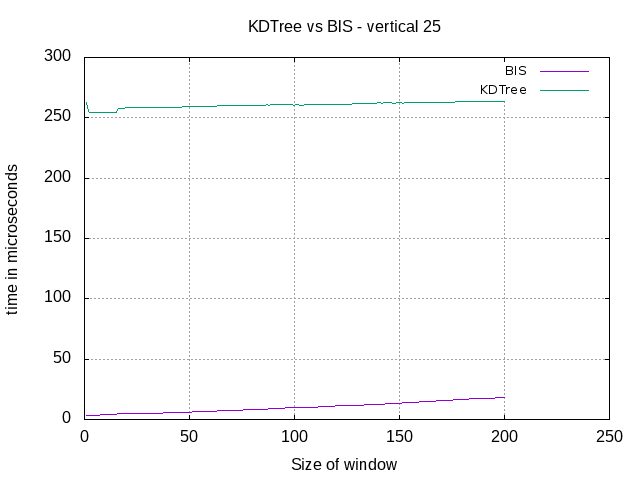
\includegraphics[width=0.99\textwidth]{pictures/analysis/smalls/vert_25.png}
        \caption{Data set of size $n=2^{25}$.}
        \label{fig:small_vert_25}
    \end{subfigure}
  }
    \caption{Vertical slice on BIS and kd-tree.}
    \label{fig:small_vert_17_25}
  
\end{figure}

The running time of a slice to the BIS data structure where $k \leq 200$ is noticably better than the running time of a slice to the kd-tree. The figures show that the BIS data structure performs better when the size of the slice is below $200$. Seeing this tendency, we are then also interested in testing just how much better the BIS data structure performs. We are going to meassure this by testing the factor between the performance of the BIS data structure and the performance of the kd-tree. We see the result of these tests on figure~\ref{fig:small_vert_fac_17} and figure~\ref{fig:small_vert_fac_25}.



\begin{figure}[h]
  \makebox[\linewidth][c]{
    \centering
    \begin{subfigure}[b]{0.68\textwidth}
        \centering
        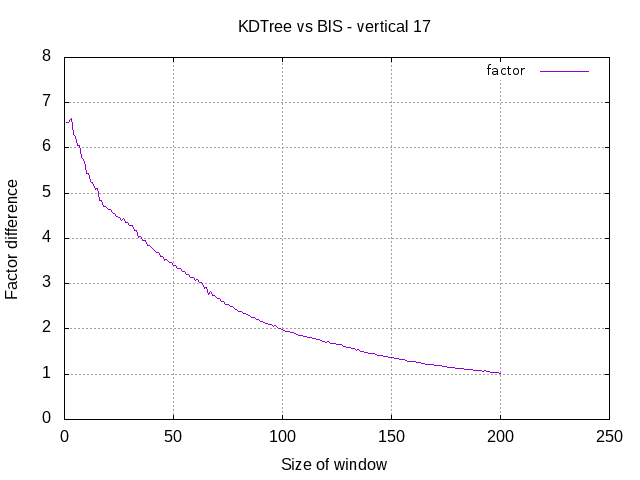
\includegraphics[width=0.99\textwidth]{pictures/analysis/smalls/vert_fac_17.png}
        \caption{Data set of size $n=2^{17}$.}
        \label{fig:small_vert_fac_17}
    \end{subfigure}
    %\hfill
    \begin{subfigure}[b]{0.68\textwidth}
        \centering
        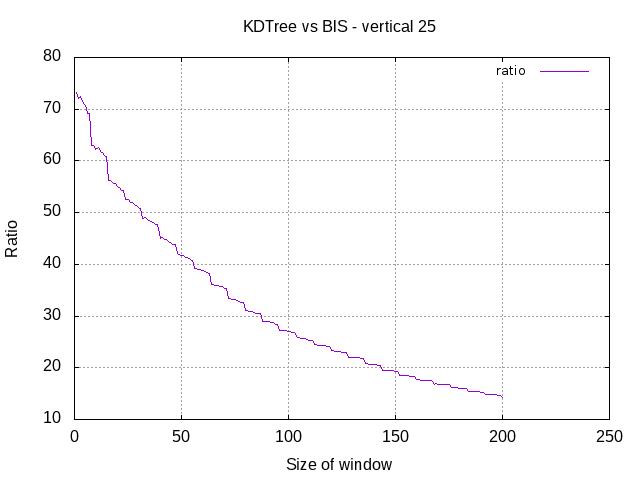
\includegraphics[width=0.99\textwidth]{pictures/analysis/smalls/vert_fac_25.png}
        \caption{Data set of size $n=2^{25}$.}
        \label{fig:small_vert_fac_25}
    \end{subfigure}
  }
    \caption{Ratio between running time of slice on BIS and kd-tree.}
    \label{fig:small_vert_fac_17_25}
  
\end{figure}
\clearpage

\todo{Skal jeg lave en graf med det? Sæt size fast og se hvordan faktoren stiger når $\lg n$ vokser?}

Looking at figure~\ref{fig:small_vert_fac_17} and figure~\ref{fig:small_vert_fac_25} we notice that the ratio between the two running times at $size = 100$ increases from $2$ to $27$. A factor of $27$ is the difference between the vertical slice to the BIS data structure and a vertical slice to the kd-tree with $size = 100$.

Looking back to the section about the square windows we remember that a window with the dimensions $\sqrt{n}\cdot{size} \times \sqrt{n}\cdot\sqrt{size}$ is expected to return $size$ points as result. This was based on the area of area of the search query. Thus, we can rewrite the expression as follows: $\sqrt{n}\cdot{size} \times \sqrt{n}\cdot\sqrt{size} = \sqrt{n}\cdot\sqrt{n} \times \sqrt{size}\cdot\sqrt{size} = n \times size$. This is exactly what vertical or horizontal slice looks like. Thus, we know that these two types of queries are expected to return the same amount of points and we can therefore compare the square search query with a horizontal or vertical slice to see how much of an impact the shape of the search has for the BIS data structure.

\todo{Her ville det nok være sjovt at se hvordan de to data strukturer sammenligner - enten vis $\frac{slice-kd}{slice-BIS} + \frac{square-BIS}{square-kd}$ eller $\frac{kd-square}{kd-slice} + \frac{BIS-slice}{BIS-square}$ og vis hvilken der klarer sig bedst med at omstille sig. Bare en eller anden måde at vise vores datastruktur ikke bliver såå smadret af at ændre form. Måske kigge på noget der er større end bare 100.}

We pick $size=\{50,100,150\}$ from both the squared tests and the slices to see how changing the shape of the query affects the running time of the query to the BIS data structure. The graphs on figure~\ref{fig:all_50}, figure~\ref{fig:all_100} and figure~\ref{fig:all_150} show some similarities. The vertical slice is clearly the fastest. The horizontal slice performs worse than the vertical slice. The squared window search query seems to be the worst-case scenario for the BIS data structure. But looking at only the squared window search across the three graphs we see that it growing with a rather linear tendency. We would expect as much from the theory because if we fix $k$ in $\mathcal{O}(\lg n + k\cdot \lg^\epsilon n$ we only have $\lg n$ and $lg^\epsilon n$ growing. Since $\lg n$ increases by $1$ and $\mathcal{O}(lg^\epsilon n)$ is a bound for the amount of jumps performed, this ties rather well to the theory. Looking at these three graphs, we suspect that the squared window search is the general case of a search query to the BIS data structure, while both the horizontal and vertical slice searches are special cases performing even better. \todo{Det er tydeligt fra teorien - og forklaringen ovenfor - at vertical er det bedste. Hvorfor er horizontal bedre end sqrt?}. Thus, the time required to find $k$ points with a search query to the BIS data structure is bound by a graph growing linearly to $\lg n$. 


\begin{figure}[h]
  \makebox[\linewidth][c]{
    \centering
    \begin{subfigure}[b]{0.68\textwidth}
        \centering
        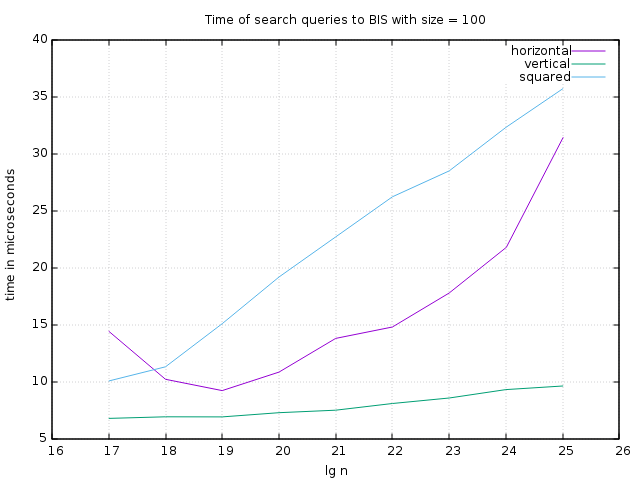
\includegraphics[width=0.99\textwidth]{pictures/analysis/smalls/all_100.png}
        \caption{Queries to the BIS data structure with $size=100$.}
        \label{fig:all_100}
    \end{subfigure}
    %\hfill
    \begin{subfigure}[b]{0.68\textwidth}
        \centering
        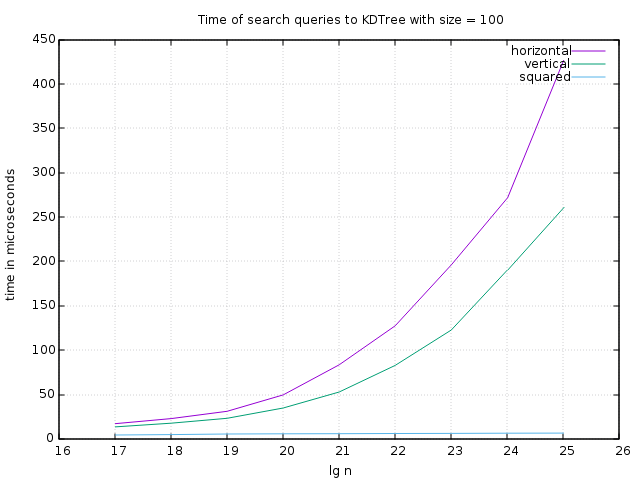
\includegraphics[width=0.99\textwidth]{pictures/analysis/smalls/all_kdtree_100.png}
        \caption{Queries to the kd-tree with $size=100$.}
        \label{fig:all_kdtree_100}
    \end{subfigure}
  }
  \caption{Comparison of shapes on BIS and KDtree.}
  \label{fig:all_100_and_kdtree}
  
\end{figure}

\begin{figure}[h]
  \makebox[\linewidth][c]{
    \centering
    \begin{subfigure}[b]{0.68\textwidth}
        \centering
        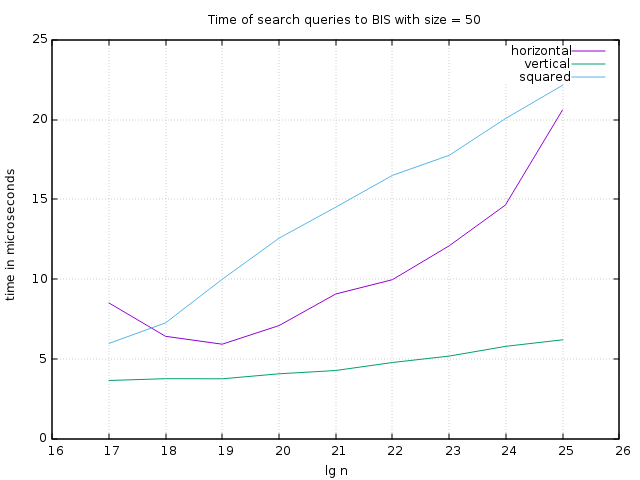
\includegraphics[width=0.99\textwidth]{pictures/analysis/smalls/all_50.png}
        \caption{Queries to the BIS data structure with $size=50$.}
        \label{fig:all_50}
    \end{subfigure}
    %\hfill
    \begin{subfigure}[b]{0.68\textwidth}
        \centering
        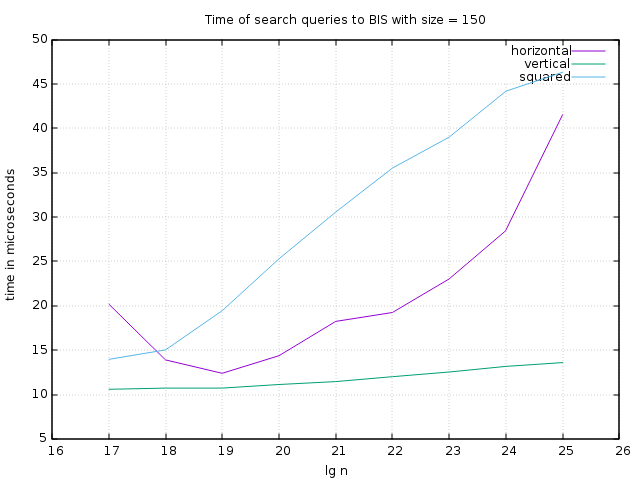
\includegraphics[width=0.99\textwidth]{pictures/analysis/smalls/all_150.png}
        \caption{Queries to the kd-tree with $size=150$.}
        \label{fig:all_150}
    \end{subfigure}
  }
  \caption{Comparison of shapes on BIS.}
  \label{fig:all_50_and_150}
  
\end{figure}


We look at figure~\ref{fig:all_kdtree_100} in order to confirm changing the shape from a squared window to a slice impacts the time of the search query to kd-tree in a much bigger way than changing the shape of the search query to the SRS data structure.

In section~\ref{sect:squares} we found the ratio between a square query to the kd-tree and a square query to the BIS data structure in order to find out how much better the kd-tree performed. Now the roles are reversed, and we are now interested in seeing how much better the BIS data structure performs. 


\begin{figure}[h]
  \makebox[\linewidth][c]{
    \centering
    \begin{subfigure}[b]{0.68\textwidth}
        \centering
        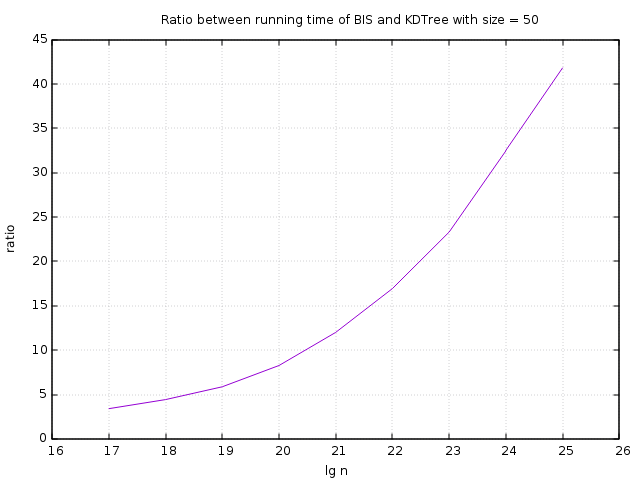
\includegraphics[width=0.99\textwidth]{pictures/analysis/factor_difference_vert_50.png}
        \caption{Ratio with $size=50$.}
        \label{fig:fact_diff_vert_50}
    \end{subfigure}
    %\hfill
    \begin{subfigure}[b]{0.68\textwidth}
        \centering
        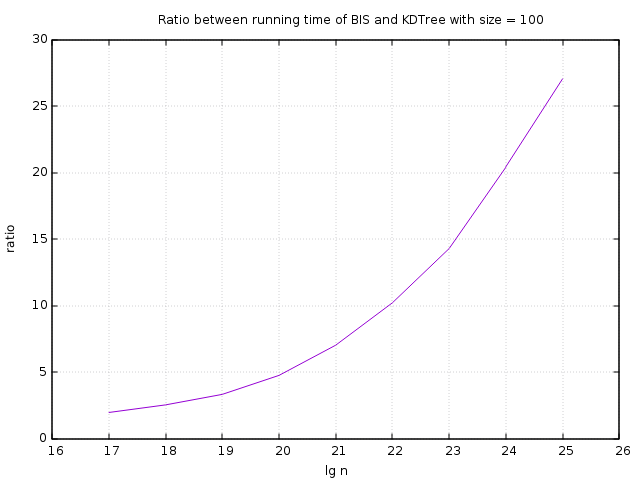
\includegraphics[width=0.99\textwidth]{pictures/analysis/factor_difference_vert_100.png}
        \caption{Ratio with $size=100$.}
        \label{fig:fact_diff_vert_100}
    \end{subfigure}
  }
  \caption{Ratio between BIS data structure and kd-tree. Describes how much better the BIS data structure performs compared to the kd-tree.}
  \label{fig:fact_diff_vert_50_100}
  
\end{figure}


\begin{figure}[h]
    \centering
    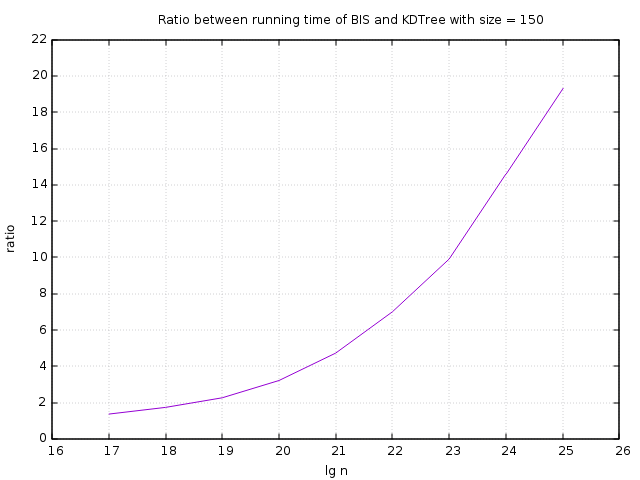
\includegraphics[width = 0.85\textwidth]{pictures/analysis/factor_difference_vert_150.png}
    \caption{Ratio between BIS data structure and kd-tree with $size=150$. Describes how much better the BIS data structure performs compared to the kd-tree.}\label{fig:fact_diff_vert_150}
\end{figure}
\clearpage



\section{Comparison of the different SRS data structures with $B$ varying}

So far we have only looked at the BIS data structure with $B = \lceil \frac{1}{2}\lg^{\frac{1}{3}} n \rceil = 2$. We have also not yet mentioned the important aspect of how much main memory the BIS data structure uses compared to the kd-tree. In this section we are going to look at the BIS data structure with $B = \lceil c \cdot \lg^\epsilon n \rceil$ where $c$ and $\epsilon$ is chosen such that $B={2,3,4}$ and show how space it uses and compare it to the space used by the kd-tree. We will also look at how well the vertical and horizontal slices perform with $B={3,4}$ by looking at when the query time for a search query to SRS data structure instersects the query time for a search query to the kd-tree.

We are going to briefly look at how the BIS data structure performs with $B=\{3,4\}$. Again, we are going to focus on the vertical slices. We start by introducing figure~\ref{fig:3vert} to see at what size the running time of vertical slices to the BIS data structure with $B=3$ intersects with the running time of the same query to the kd-tree. Recall we have already seen these graphs for $B=2$ on figure~\ref{fig:vert_intersection}.

We are going to introduce the exact same graphs for $B=4$. These are seen on figure~\ref{fig:4vert}.



\begin{figure}[h]
  \makebox[\linewidth][c]{
    \centering
    \begin{subfigure}[b]{0.68\textwidth}
        \centering
        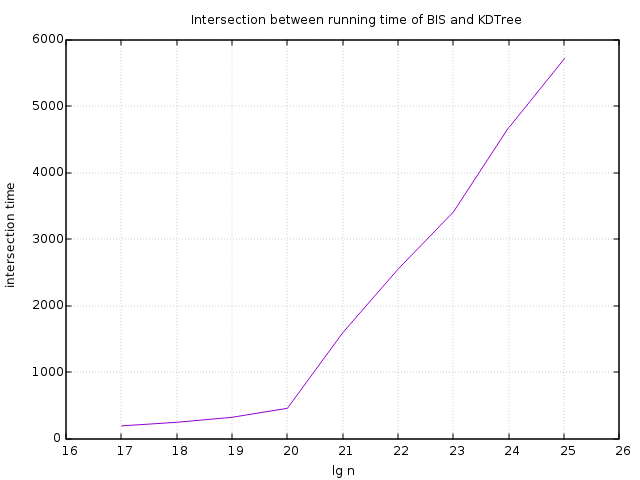
\includegraphics[width=0.99\textwidth]{pictures/analysis/threes/vert.png}
        \caption{Point of intersection with $B=3$.}
        \label{fig:3vert}
    \end{subfigure}
    %\hfill
    \begin{subfigure}[b]{0.68\textwidth}
        \centering
        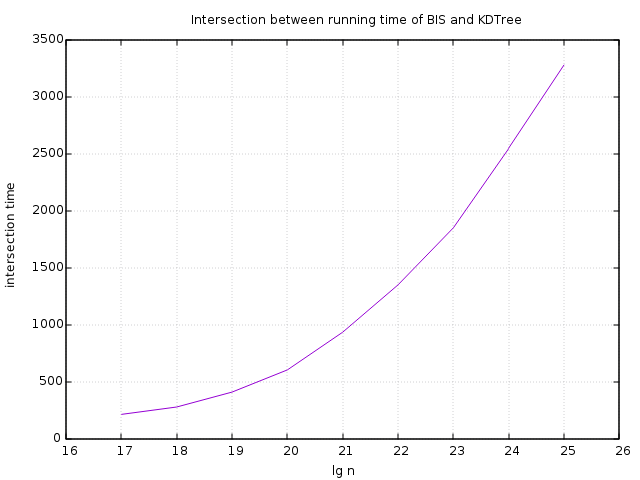
\includegraphics[width=0.99\textwidth]{pictures/analysis/fours/vert.png}
        \caption{Point of intersection with $B=4$.}
        \label{fig:4vert}
    \end{subfigure}
  }
  \caption{Ratio between BIS data structure and kd-tree. Describes how much better the BIS data structure performs compared to the kd-tree.}
  \label{fig:34vert}
  
\end{figure}

\begin{figure}[h]
  \makebox[\linewidth][c]{
    \centering
    \begin{subfigure}[b]{0.68\textwidth}
        \centering
        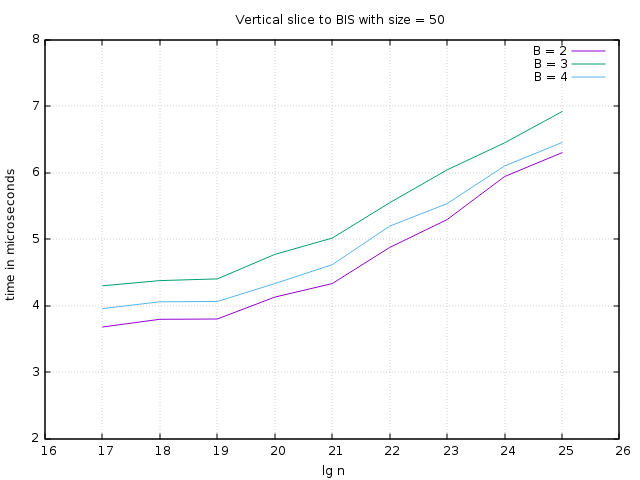
\includegraphics[width=0.99\textwidth]{pictures/analysis/comparing_BIS_50.png}
        \caption{BIS with $size = 50$.}
        \label{fig:BIS_50}
    \end{subfigure}
    %\hfill
    \begin{subfigure}[b]{0.68\textwidth}
        \centering
        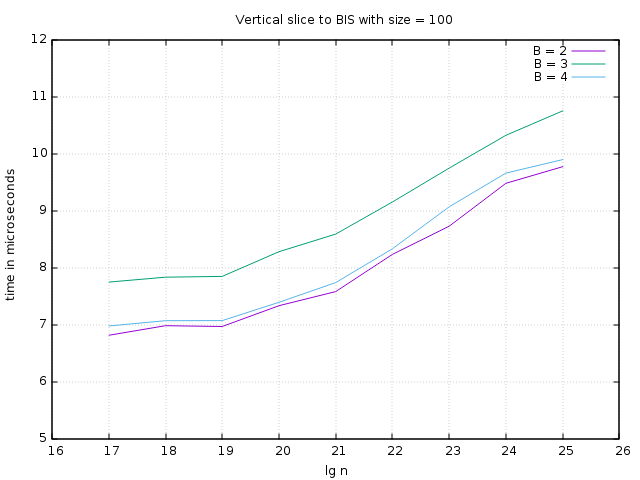
\includegraphics[width=0.99\textwidth]{pictures/analysis/comparing_BIS_100.png}
        \caption{BIS with $size = 100$.}
        \label{fig:BIS_100}
    \end{subfigure}
  }
  \caption{BIS with $B = \{2,3,4\}$. Comparing vertical slices to each}
  \label{fig:comparing_BIS}
  
\end{figure}


The most important reason why the range tree is not used as the standard range reporting data structure today is its space complexity. While we have shown theoretically that the space complexity of the BIS data structure is linear, we would also like to see it in practice. Figure~\ref{fig:sizes} shows the actual space usage of the BIS data structure with $B=\{2,3,4\}$ and the space usage of the kd-tree. The size has been normalized by the amount of points the data structure holds. Thus, the normalized size of the kd-tree is $2$, meaning that for each point in the kd-tree it uses $2\cdot 32$ bits - one $32$ bits integer for each coordinate.

\begin{figure}[h]
    \centering
    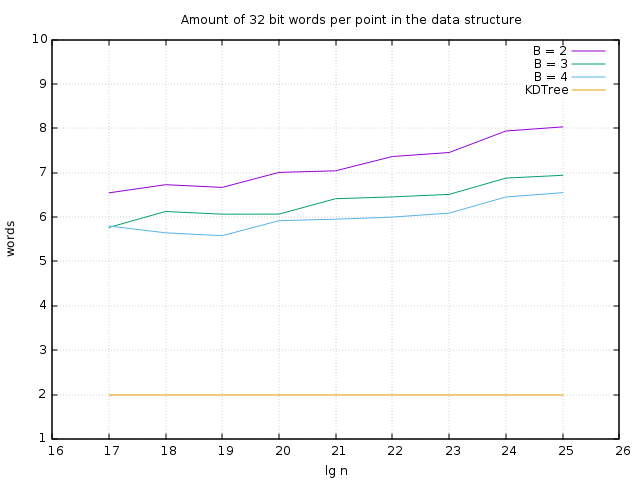
\includegraphics[width = 0.85\textwidth]{pictures/analysis/sizes.png}
    \caption{The normalized sizes of the BIS data structure with $B=\{2,3,4\}$ and the kd-tree.}\label{fig:sizes}
\end{figure}
\clearpage


An interesting thing to note is that the size of the kd-tree is entirely dependent on the data type used to represent each coordinate. In our experiements we have used a $32$ bit unsigned integer. If we were to change that to a $64$ bit unsigned integer, the size of the kd-tree would increase by a factor of $2$. As the kd-tree, the BIS data structure uses $2$ words per point to store the coordinates. The BIS data structure also uses $1$ word per point to store the y-coordinates in a sorted list as to allow for binary search to find $\hat{y_1}$ and $\hat{y_2}$. The rest of the BIS data structure are no dependent on the data type used to represent the coordinates. Thus, changing the data type from a $32$ bit integer to a $64$ bit integer would only increase the total space usage by $3$. On figure~\ref{fig:sizes} the size of the BIS data structure with $B=2$ and $\lg n = 25$ is $8$. Increasing that to $11$ would increase the space usage of the BIS data structure by a factor of $\frac{11}{8} = 1.375$. \todo{Måske slettes}


\section{Vertical and horizontal slices explained}
\label{sect:verthoriexp}

In this we are going to dive a deeper into the results of the previous sections. The figures depicting the performance of the vertical slices showed some interesting tendencies. This is the last section before the summary and can easily be skipped.

\begin{figure}[h]
    \centering
    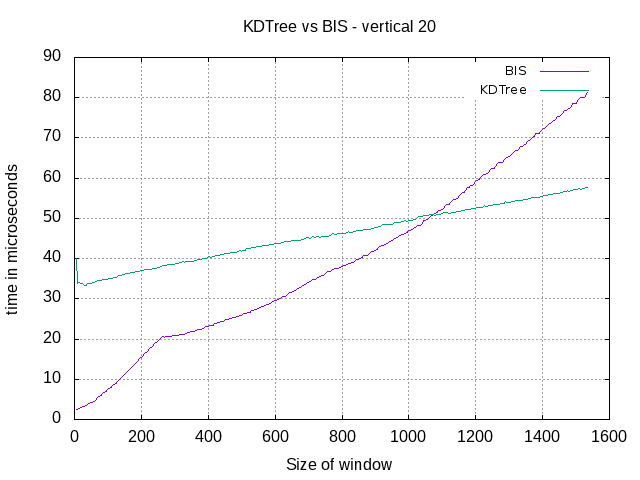
\includegraphics[width = 0.85\textwidth]{pictures/analysis/vert_20.png}
    \caption{Vertical slice. data set size of $n=2^{20}$.}\label{fig:vert_20}
\end{figure}



\begin{figure}[h]
    \centering
    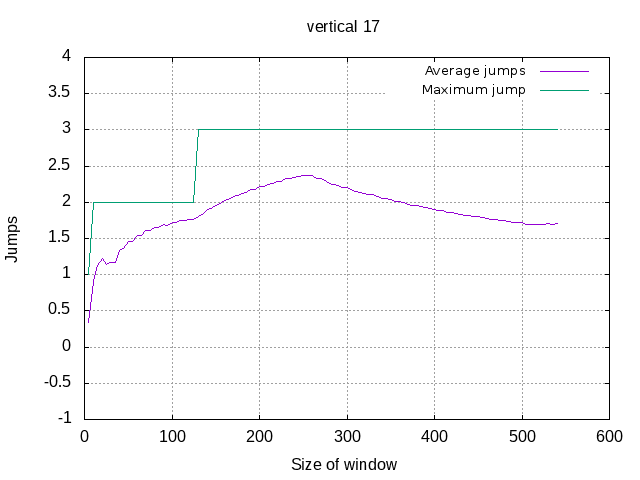
\includegraphics[width = 0.85\textwidth]{pictures/analysis/jump_vert_17.png}
    \caption{Size of jumps - data set size of $n=2^{17}$. 'Average jumps' is the average of all the jumps performed normalized by the size of the slice}\label{fig:jump_vert_17}
\end{figure}

\begin{figure}[h]
    \centering
    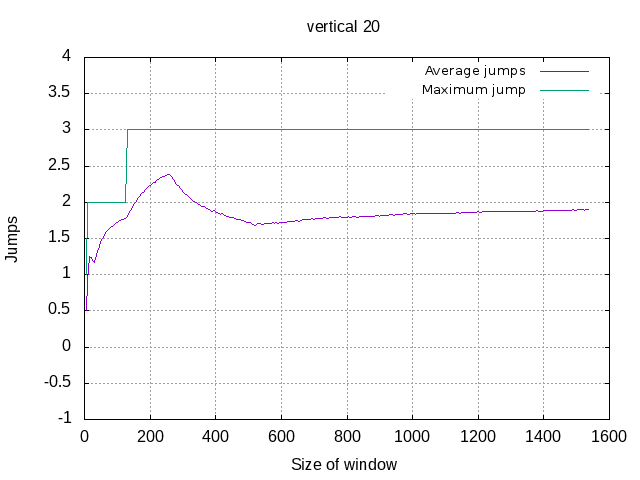
\includegraphics[width = 0.85\textwidth]{pictures/analysis/jump_vert_20.png}
    \caption{Size of jumps - data set size of $n=2^{20}$. 'Average jumps' is the average of all the jumps performed normalized by the size of the slice}\label{fig:jump_vert_20}
\end{figure}



\begin{figure}[h]
    \centering
    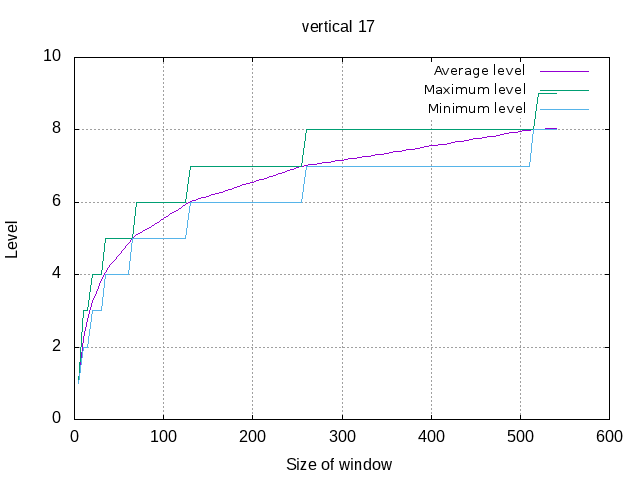
\includegraphics[width = 0.85\textwidth]{pictures/analysis/level_vert_17.png}
    \caption{Level of first fully contained node - data set size of $n=2^{17}$.}\label{fig:level_vert_17}
\end{figure}

\begin{figure}[h]
    \centering
    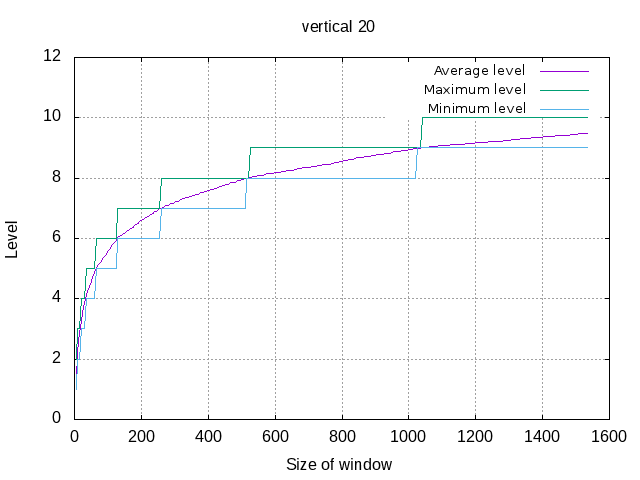
\includegraphics[width = 0.85\textwidth]{pictures/analysis/level_vert_20.png}
    \caption{Level of first fully contained node - data set size of $n=2^{20}$.}\label{fig:level_vert_20}
\end{figure}


Across the graphs showing the performance of the vertical slices to the BIS data structure, there is a very noticable change in slope at around $k=256$. Since $B=2$, we have a big jump at level $2^3 = 8$ which allows the ball inheritance structure to jump from level $8$ to a leaf in one jump. This means that the average amount of jumps per result will decrease and thus the running time will not increase as fast as before. At around $k=512$ the running-time resumes its normal behaviour. On average, the ball inheritance structure does not use the big jump at level $8$ directly anymore, resulting in a couple of steps before reaching level $8$. Since the graph shows the average run-time of different configurations of the same slice on different data sets, not all of the searches will hit level $8$ from $k>256$, but the main tedency is to. \todo{forklar tidligere - at vi snakker om main tendency, ikke hvad den er garanteret at gøre}. This tendency is described at figure~\ref{fig:jump_vert_17} and figure~\ref{fig:jump_vert_20}. We see how the graph has a local maximum at around $k=256$ and then the average amount of jumps per result decreases until $k=512$ where it starts increasing at steady level again. Figure~\ref{fig:level_vert_17} and figure~\ref{fig:level_vert_20} describes the highest level of a fully contained node. We see between $k=256$ and $k=512$ that the maximum is level $8$ and the minimum is level $7$ and that the average level increases meaning more and more fully contained node starts using level $8$. Since we $B=2$, there is a $2$-jump every $2$ levels, a $4$-jump every $4$ levels, a $8$-jump every $8$ levels and a $16$-jump every $16$ levels. This means that level $7$ the ball inheritance structure needs $3$ jumps to reach a leaf. This is why such a noticable local maximum exits on figure~\ref{fig:jump_vert_17} and figure~\ref{fig:jump_vert_20}. The jumps per results eases off because from level $8$ there is $1$ jump, from level $9$ there are $2$ jumps and from level $10$ there are $2$ jumps. Levels $11, 13, 14$ have $3$ jumps, and at level $15$ another local maximum is going to be found with $4$ jumps, just before level $16$ with $1$ jump to the leaves. However, $k=2^{16}=65,536$ is not likely to be a place where the SRS data structure performs better than the kd-tree unless we have a enormous data set \todo{regn på det}. \todo{Sæt grafer ind for større $n$}


Looking at figure~\ref{fig:level_vert_17} we see that when we reach $k=256$ the minimum highest level rises to $7$ and the maximum highest level rises to $8$. In order to write the sum of $256<k<512$ we will need to at least level $7$ because we need the two fully included nodes from level $7$ giving us $2*2^7 = 2^8 = 256$ nodes. If the least common ancestor is found at level $9$ the first fully contained node can be found at level $7$. If all the levels from level $7$ to level $1$ only have fully contained nodes, we get $k = 2*2^1 + 2*2^2 + \cdots + 2*2^7 = 508$. This is not enough to write $512$, and thus somewhere between $k=256$ and $k=512$, the search algorithm will begin using level $10$ as the least common ancestor. This is also very dependent on how the slice covers the subtrees of the least common ancestor. If the slice hits the least common ancestor right in the middle, such that the left subtree and the right subtree of the least common ancestor is of the exact same size, the level of the highest fully included node will be lower. If the slice hits the least common ancestor such there is an imbalance in the size between the left subtree and right subtree of the least common ancestor, the level of the highest fully included node will be higher, because now one subtree has to account for a bigger portion of the slice and will have to use bigger pieces. And when a subtree contains $2^8 = 256$ leaves it will have access to the jump at level $8$. The maximum level of figure~\ref{fig:level_vert_17} is explained by the fact that it is not possible to write the sum of $k<512$ using $512$ as a summand. Recall that a vertical slice conceptually only searches for the x-coordinates of the points. All the y-coordinates are already known to be included, Thus, when a node is fully included, we get all of points in its subtree.   \todo{Omformuler og sæt sammen med afsnittet fra før lige ovenover da du skriver nogenlunde det samme - bare i to forskellige tankegange}\todo{Lav en lignede figur som figur 3.2 til at forklare konceptet}

As mentioned before, it is hard to argue about the tendencies of the graphs of the horizontal slices. When the least common ancestor of $x_1$ and $x_2$ is found at level $i$, the first node which is fully contained in a horizontal slice is located on level $i-2$. So from level $i-1$ to level $1$ we find $2$ fully contained nodes per level. The points are uniformly distributed which means that given one y-rank the chance to find it on level $i-2$ is $2\cdot\frac{1}{4} = \frac{1}{2}$. The chance to find it on level $i-3$ is half that, i.e. $\frac{1}{4}$. Thus, when we see the graphs of the horizontal slices.. bla bla

\begin{figure}[h]
    \centering
    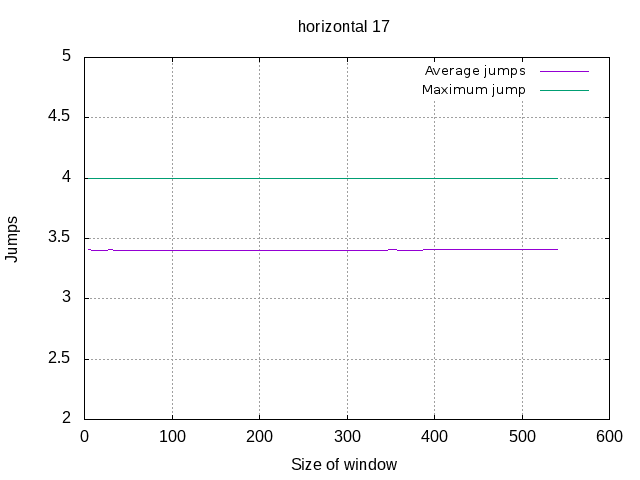
\includegraphics[width = 0.85\textwidth]{pictures/analysis/jump_hori_17.png}
    \caption{Size of jumps - data set size of $n=2^{17}$. 'Average jumps' is the average of all the jumps performed normalized by the size of the slice}\label{fig:jump_hori_17}
\end{figure}
\clearpage

Forklar konceptet med hvordan average jumps ser ud. This seemingly uninteresting graph shows us that the theory of the expected distribution is correct. We also had this confirmed in section~\ref{sect:squares} where we saw that square searches of size $\sqrt{n}\cdot\sqrt{k} \times \sqrt{n}\cdot\sqrt{k}]$ returned $k$ results. This was based on theory that assumed the distribution was uniform. If the y-coordinates are uniformly distributed amongst the x-coordinates to generate a point, we can see something interesting in figure~\ref{fig:jump_hori_17}. A BIS data structure with data set size $n = 2^{17}$ will have its first fully contained node at level $15$. For each y-coordinate we have to find, there is a $\frac{2}{4} = \frac{1}{2}$ chance that it will jump from level $15$. Then there is a $\frac{1}{4}$ chance that it will jump from level $14$ and so on. Given this information we can we can use table-something to see how many jumps a ball must take in order to get from a node at level $i$ to a leaf. Doing this we see that $\frac{4}{2} + \frac{3}{4} + \frac{3}{8} + \frac{2}{16} + \frac{3}{32} + \frac{2}{64} + \frac{2}{128} = 3.391$ which is the jumps per results depicted on figure~\ref{fig:jump_hori_17}. \todo{Kan jeg nu rent faktisk bruge det her til at forklare hvor hori tager de mærkelige svingninger?}

SENERE: Kig på $size = 300$ for alle $\lg n$. Se hvordan det er dårlig ved $\lg n = 17$ for der er første hop med størst sandsynlighed på level 15 som er $1+2+4+8 = 15 => 4$ hop. Ved $\lg n = 18$ er den god for der er størst sandsynlighed for $16 => 1$ hop. Når vi kommer højere f.eks. $\lg n = 24$ er første hop ved level $22 = 2 + 4 + 16$ og andet hop er $1 + 4 + 16$. Så tre hop er $\frac{3}{4}$ sandsynlighed. Sammenlign det med en hvor der er $2$ og $3$, f.eks. $\lg n = 22$.
\todo{Forklar om hvordan distribution af points og hvordan hvor vi ligger i forhold til level $15$ betyder noget. Kig også på grafen for figur~\ref{fig:hori_jumps_per_lgn}. Den viser netop at $\lg n = 17$ med LCA = level $15$ er noget skidt.}


\todo{Hvorfor knækker grafen mellem $512$ og $1024$? Hvorfor er kd-træet mærkeligt dårligt inden $k=10$? HORI}





\section{Summary}

In this chapter we have presented different tests on the BIS data structure. We have compared it to the kd-tree and confirmed that the theory works well in practice.

The BIS data structure performs very well as a slice, most notably as a vertical slice. A square search query does not perform as well as a slice does on the BIS data structure. However the square search query is not a disaster on the BIS data structure. We noticed the difference in performance between the square and slice-formed search query to the BIS data structure was not as big as the difference in performance between the two shapes on the kd-tree. The worst kind of test for the kd-tree was a slice and the best was a square - the exact opposite of the BIS data structure. 

The kd-tree is much more dependent on the shape of its search query than the BIS data structure. This is most notable by looking at the difference between figure~\ref{fig:all_100} and figure~\ref{fig:all_kdtree_100}.


En spændende sammenhæng. Hvor kd-træet er dårlig er BIS god, og omvendt. kd-træet er dog stadig kun præcis lineær i tid, men BIS har en penalty pr point. Men i små punkt-mængder er BIS rent faktisk rigtig god. Forskellen mellem shapes er ikke så drastisk som kd-træet.

Hvordan adskiller de forskellige shapes sig i SRS? Vi ser at kd-træet er meget afhængig af sin shape i praksis som den er i teori. Hvordan gælder det for SRS? Hvordan adskiller de forskellige shapes fra hinanden tidsmæssigt? 
